\newpage
\addsec{Anhang}
\label{sec:Anhang}

\begin{figure}[h!]
  \centering
  
\includegraphics[width=0.85\textwidth]{data/temp/rot_ohneB_0.JPG}
  \caption{Interferenzbild der Lummer-Gehrcke Platte für die rote Spektrallinie ohne angelegtes Magnetfeld für die $\sigma$-Polarisation.}
  \label{fig:rotOhneB0}
\end{figure}
\begin{figure}[h!]
  \centering
  
\includegraphics[width=0.95\textwidth]{data/temp/rot_mitB_0.JPG}
  \caption{Interferenzbild der Lummer-Gehrcke Platte für die rote Spektrallinie mit angelegtem Magnetfeld für die $\sigma$-Polarisation.}
  \label{fig:rotMitB0}
\end{figure}

\begin{figure}[h!]
  \centering
  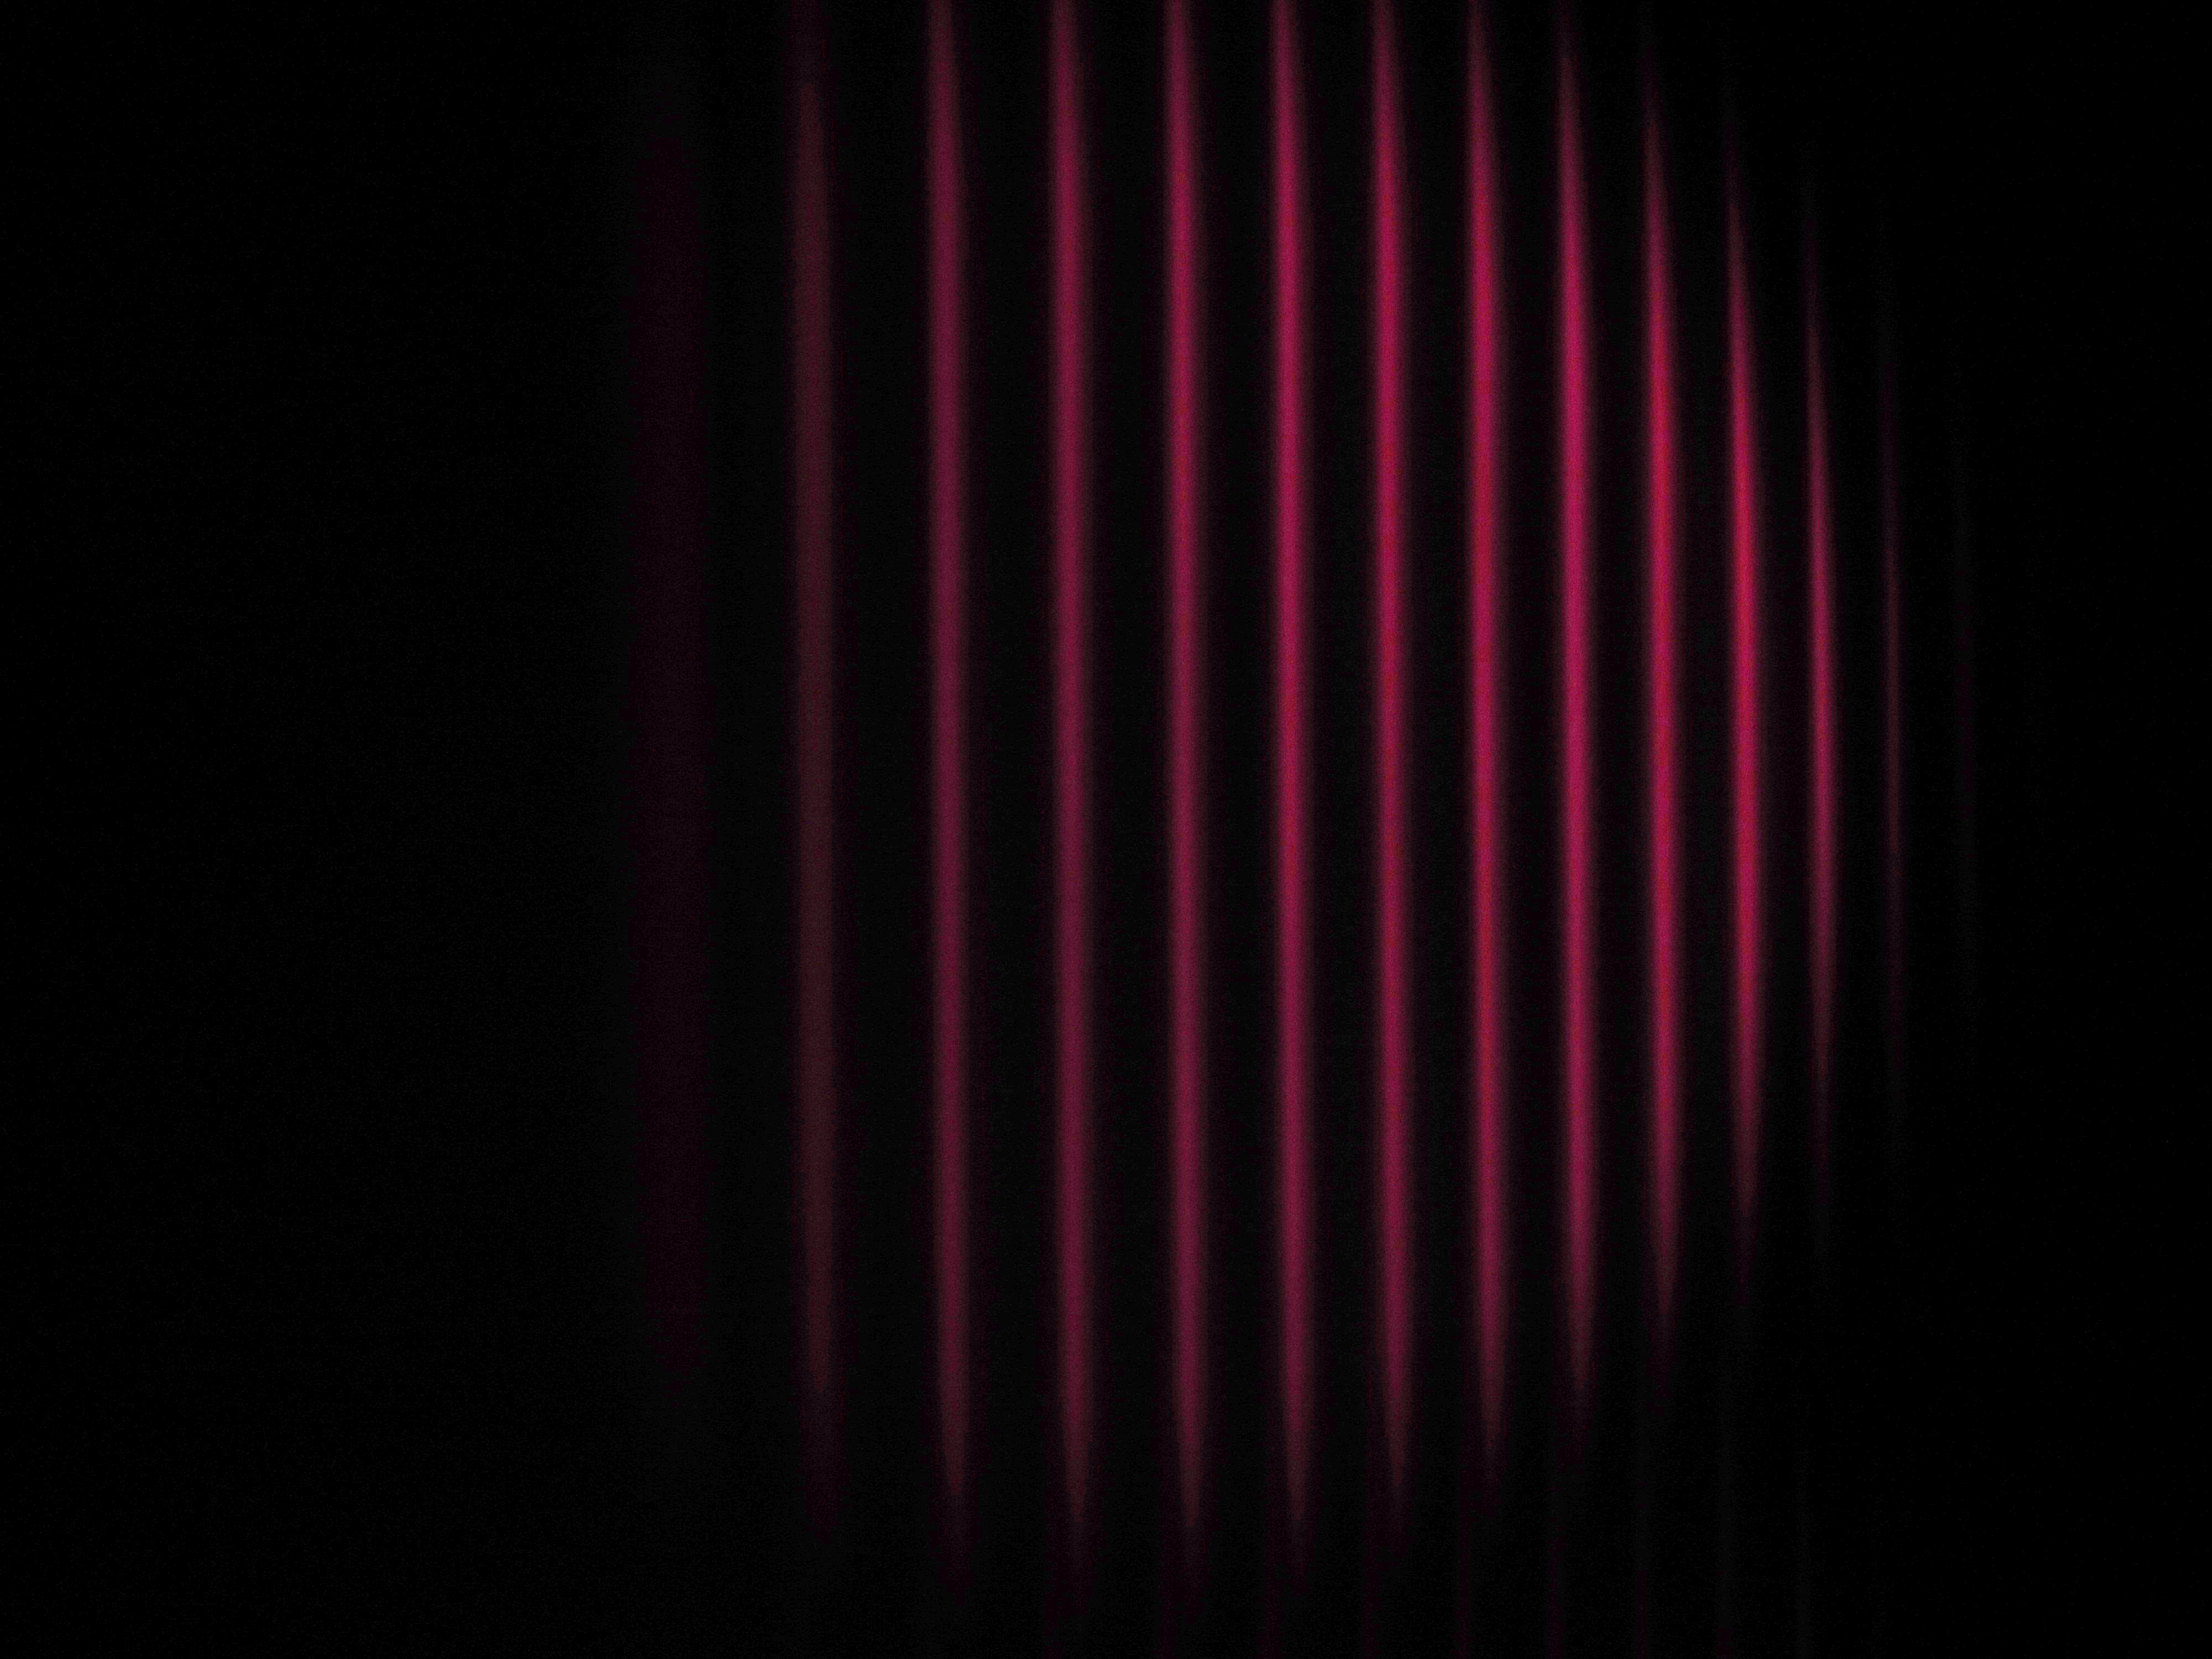
\includegraphics[width=0.85\textwidth]{data/temp/rot_ohneB_0_aufgehellt.JPG}
  \caption{Interferenzbild der Lummer-Gehrcke Platte für die rote Spektrallinie ohne angelegtes Magnetfeld für die $\sigma$-Polarisation, zur besseren Abstandsmessung mit GIMP aufgehellt.}
  \label{fig:rotOhneB0_aufgehellt}
\end{figure}
\begin{figure}[h!]
  \centering
  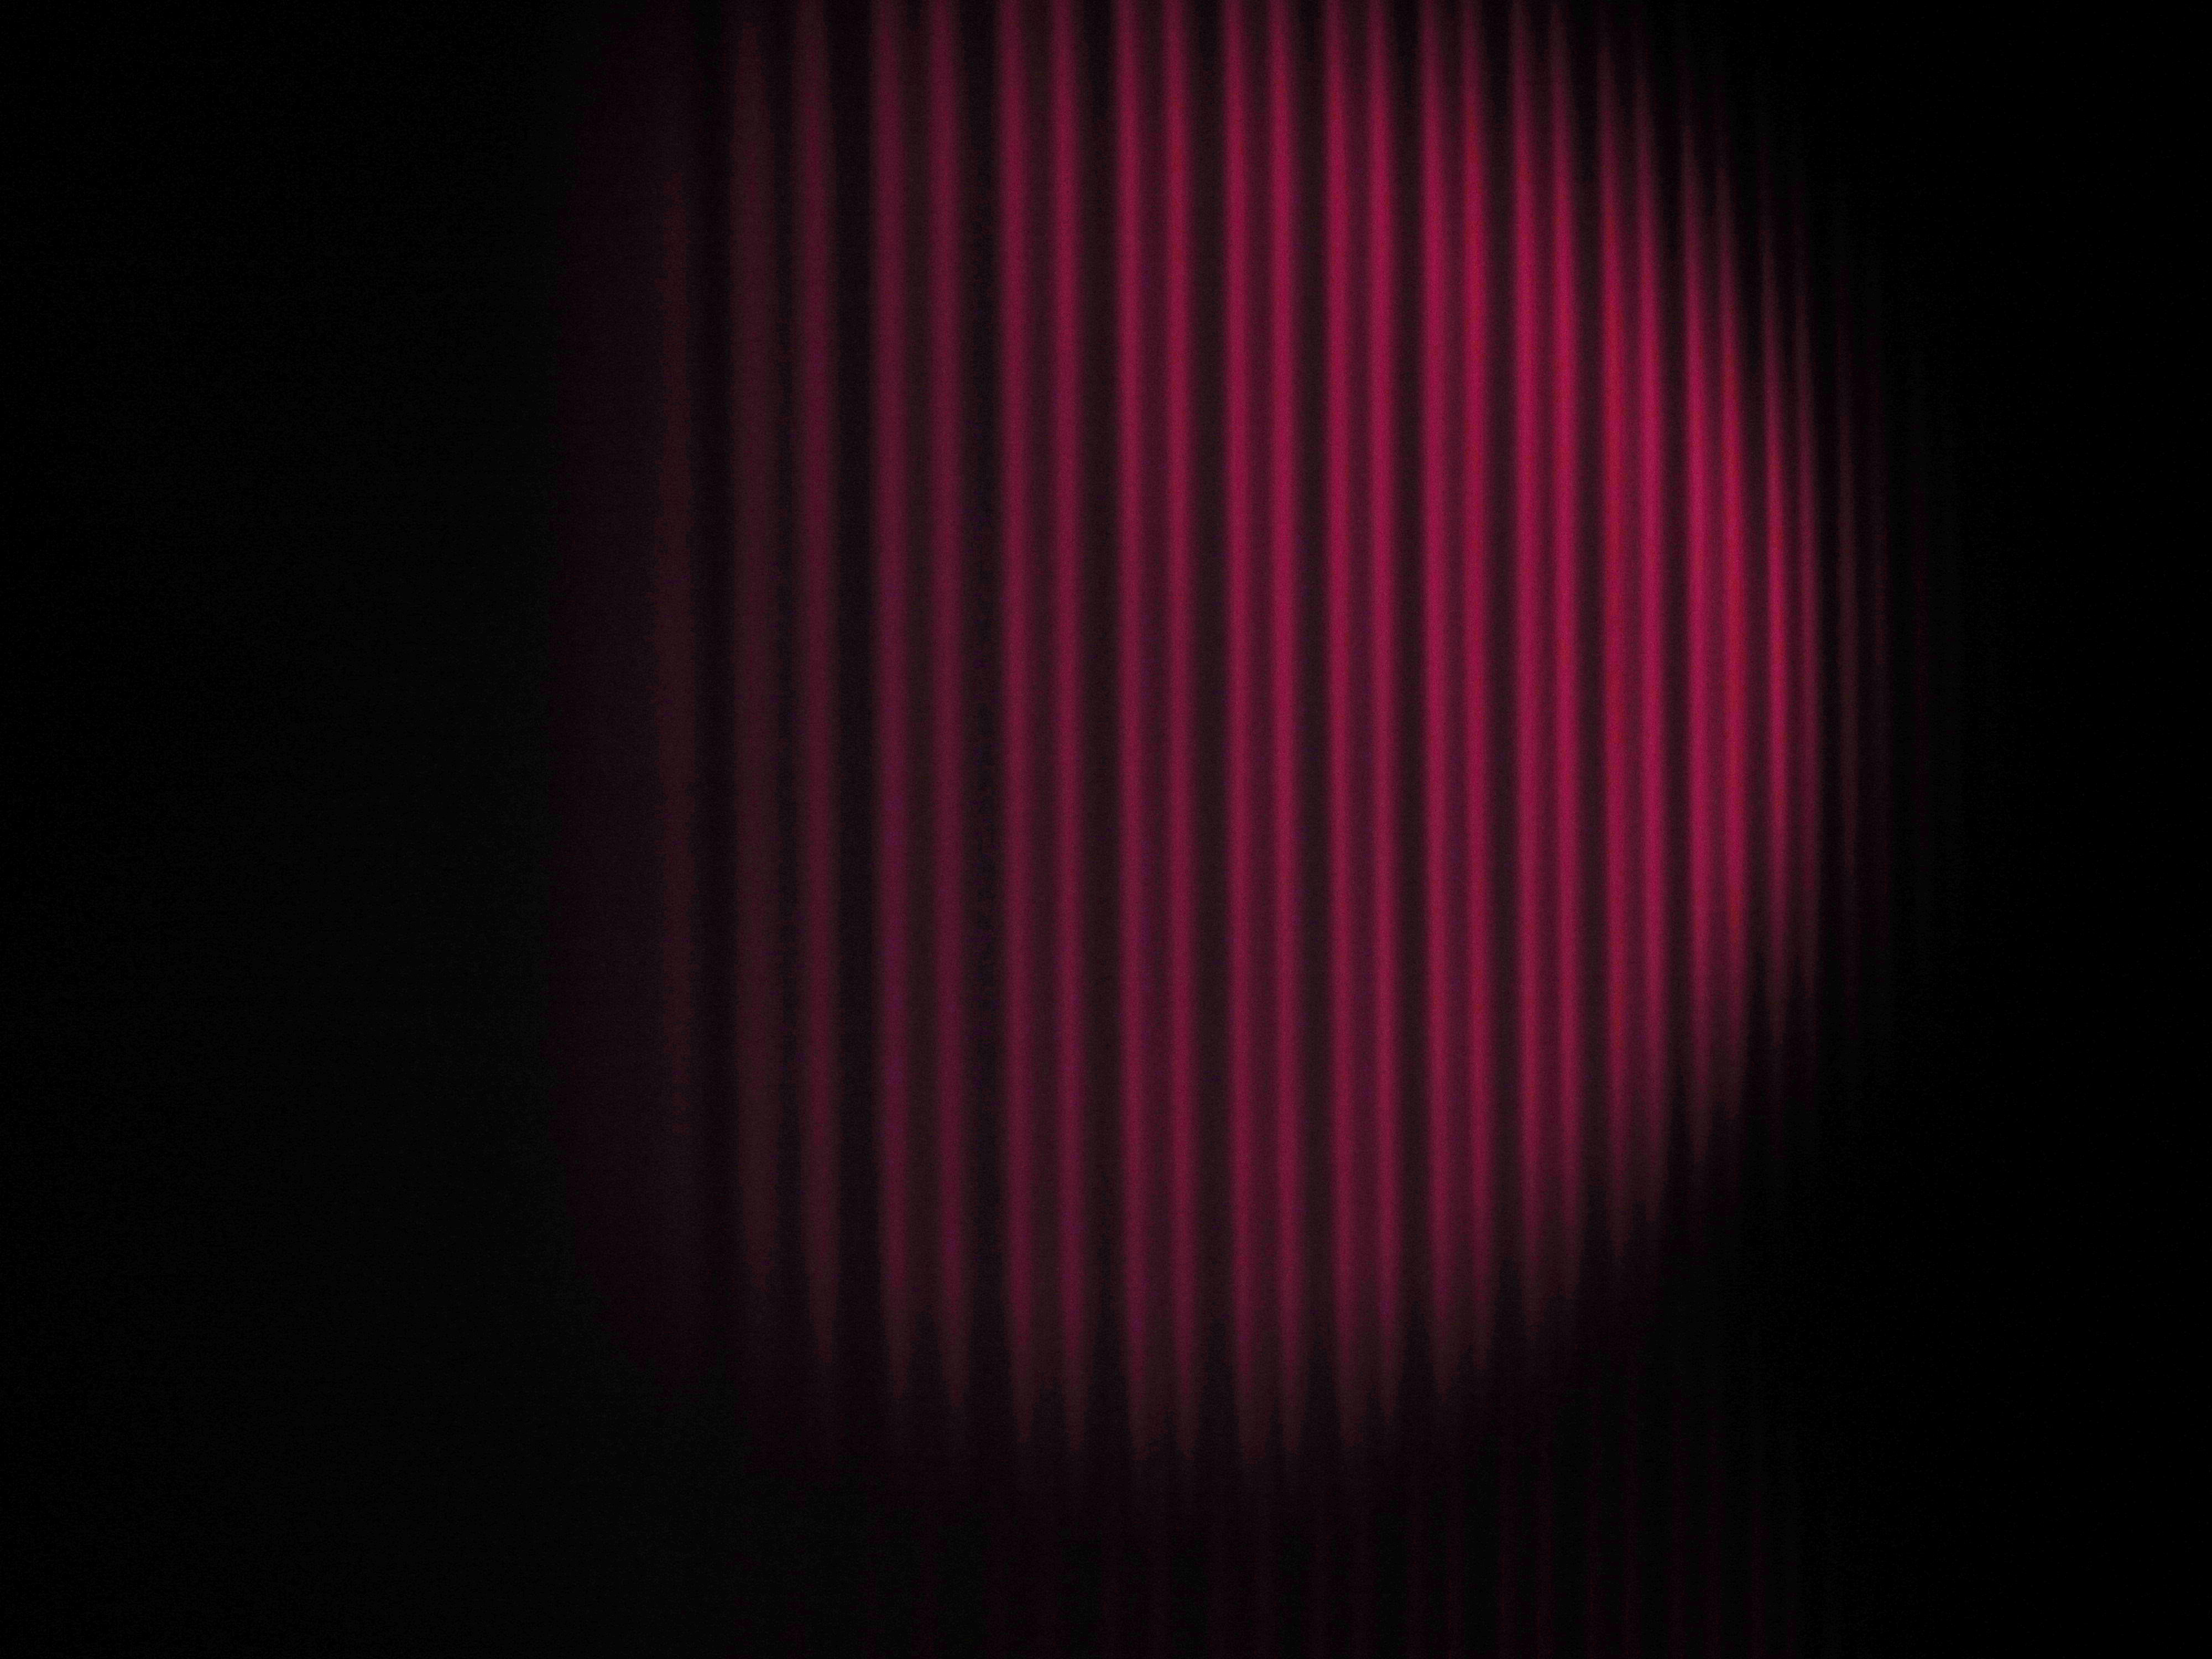
\includegraphics[width=0.95\textwidth]{data/temp/rot_mitB_0_aufgehellt.JPG}
  \caption{Interferenzbild der Lummer-Gehrcke Platte für die rote Spektrallinie mit angelegtem Magnetfeld für die $\sigma$-Polarisation, zur besseren Abstandsmessung mit GIMP aufgehellt.}
  \label{fig:rotMitB0_aufgehellt}
\end{figure}


\begin{figure}[h!]
  \centering
  
\includegraphics[width=0.85\textwidth]{data/temp/rot_ohneB_90.JPG}
  \caption{Interferenzbild der Lummer-Gehrcke Platte für die rote Spektrallinie ohne angelegtes Magnetfeld für die $\pi$-Polarisation.}
  \label{fig:roteOhneB90}
\end{figure}
\begin{figure}[h!]
  \centering
  
\includegraphics[width=0.95\textwidth]{data/temp/rot_mitB_90.JPG}
  \caption{Interferenzbild der Lummer-Gehrcke Platte für die rote Spektrallinie mit angelegtem Magnetfeld für die $\pi$-Polarisation.}
  \label{fig:rotMitB90}
\end{figure}

\begin{figure}[h!]
  \centering
  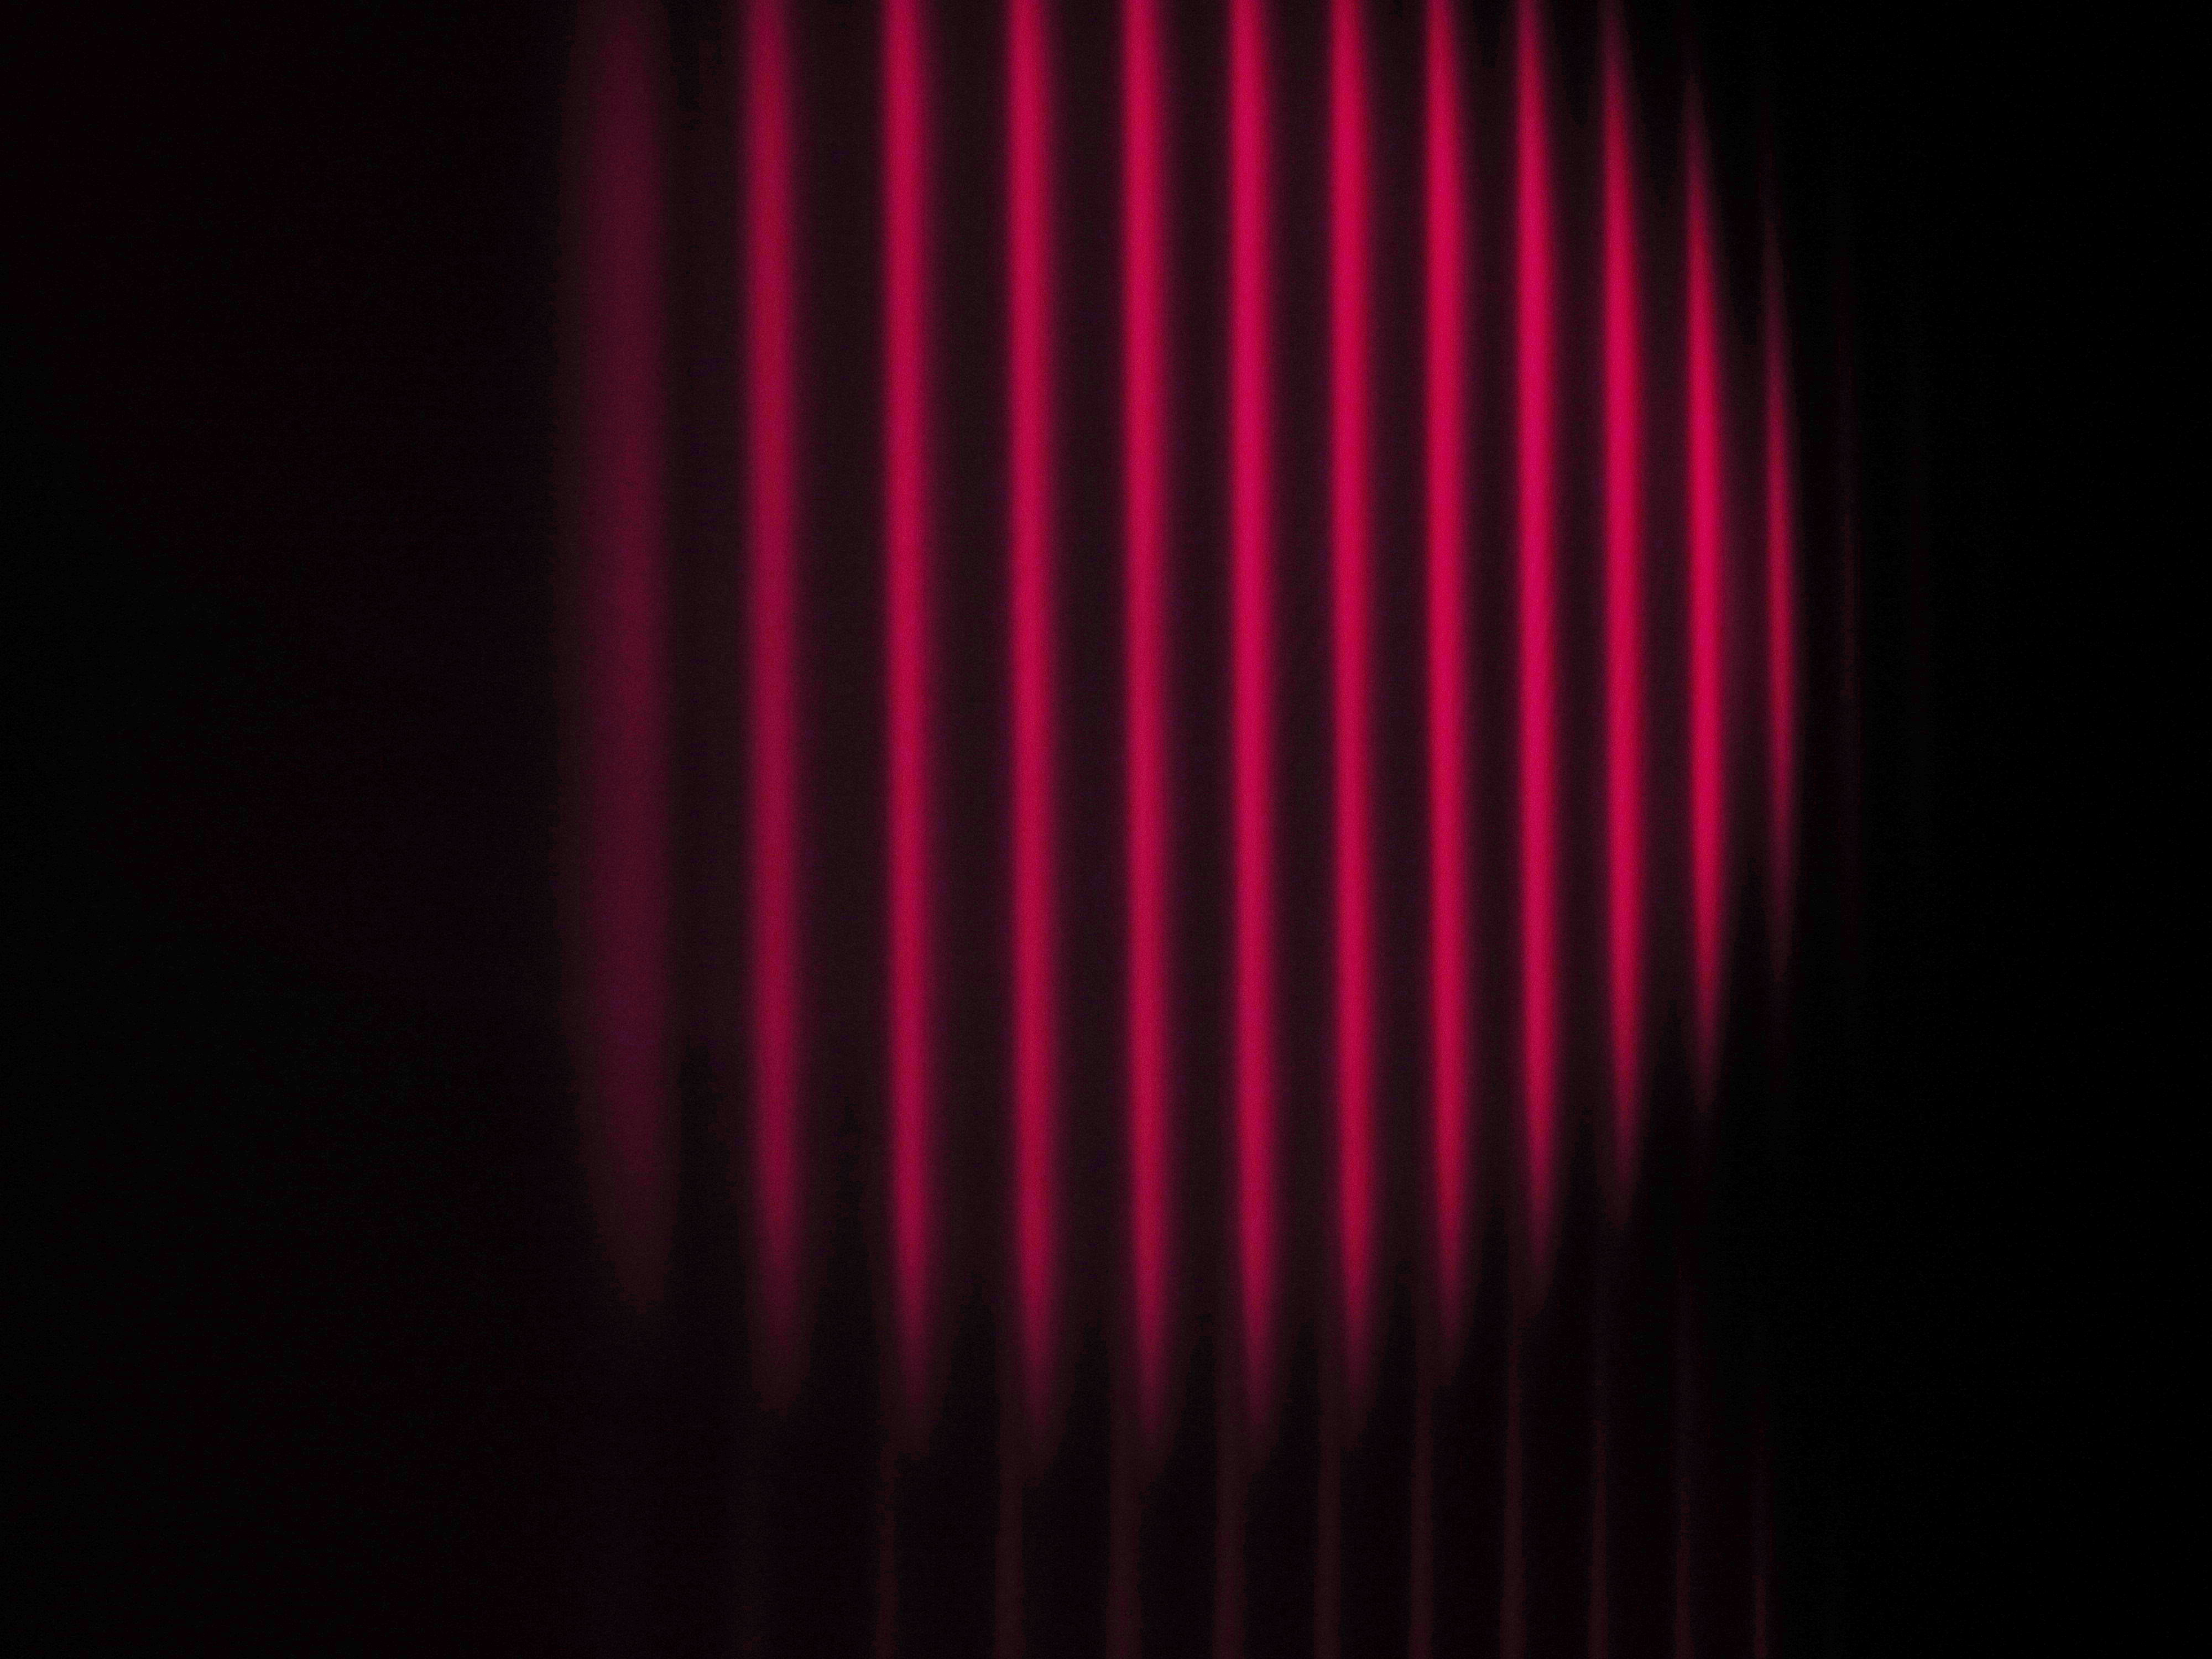
\includegraphics[width=0.85\textwidth]{data/temp/rot_ohneB_90_aufgehellt.JPG}
  \caption{Interferenzbild der Lummer-Gehrcke Platte für die rote Spektrallinie ohne angelegtes Magnetfeld für die $\pi$-Polarisation, zur besseren Abstandsmessung mit GIMP aufgehellt.}
  \label{fig:roteOhneB90_aufgehellt}
\end{figure}
\begin{figure}[h!]
  \centering
  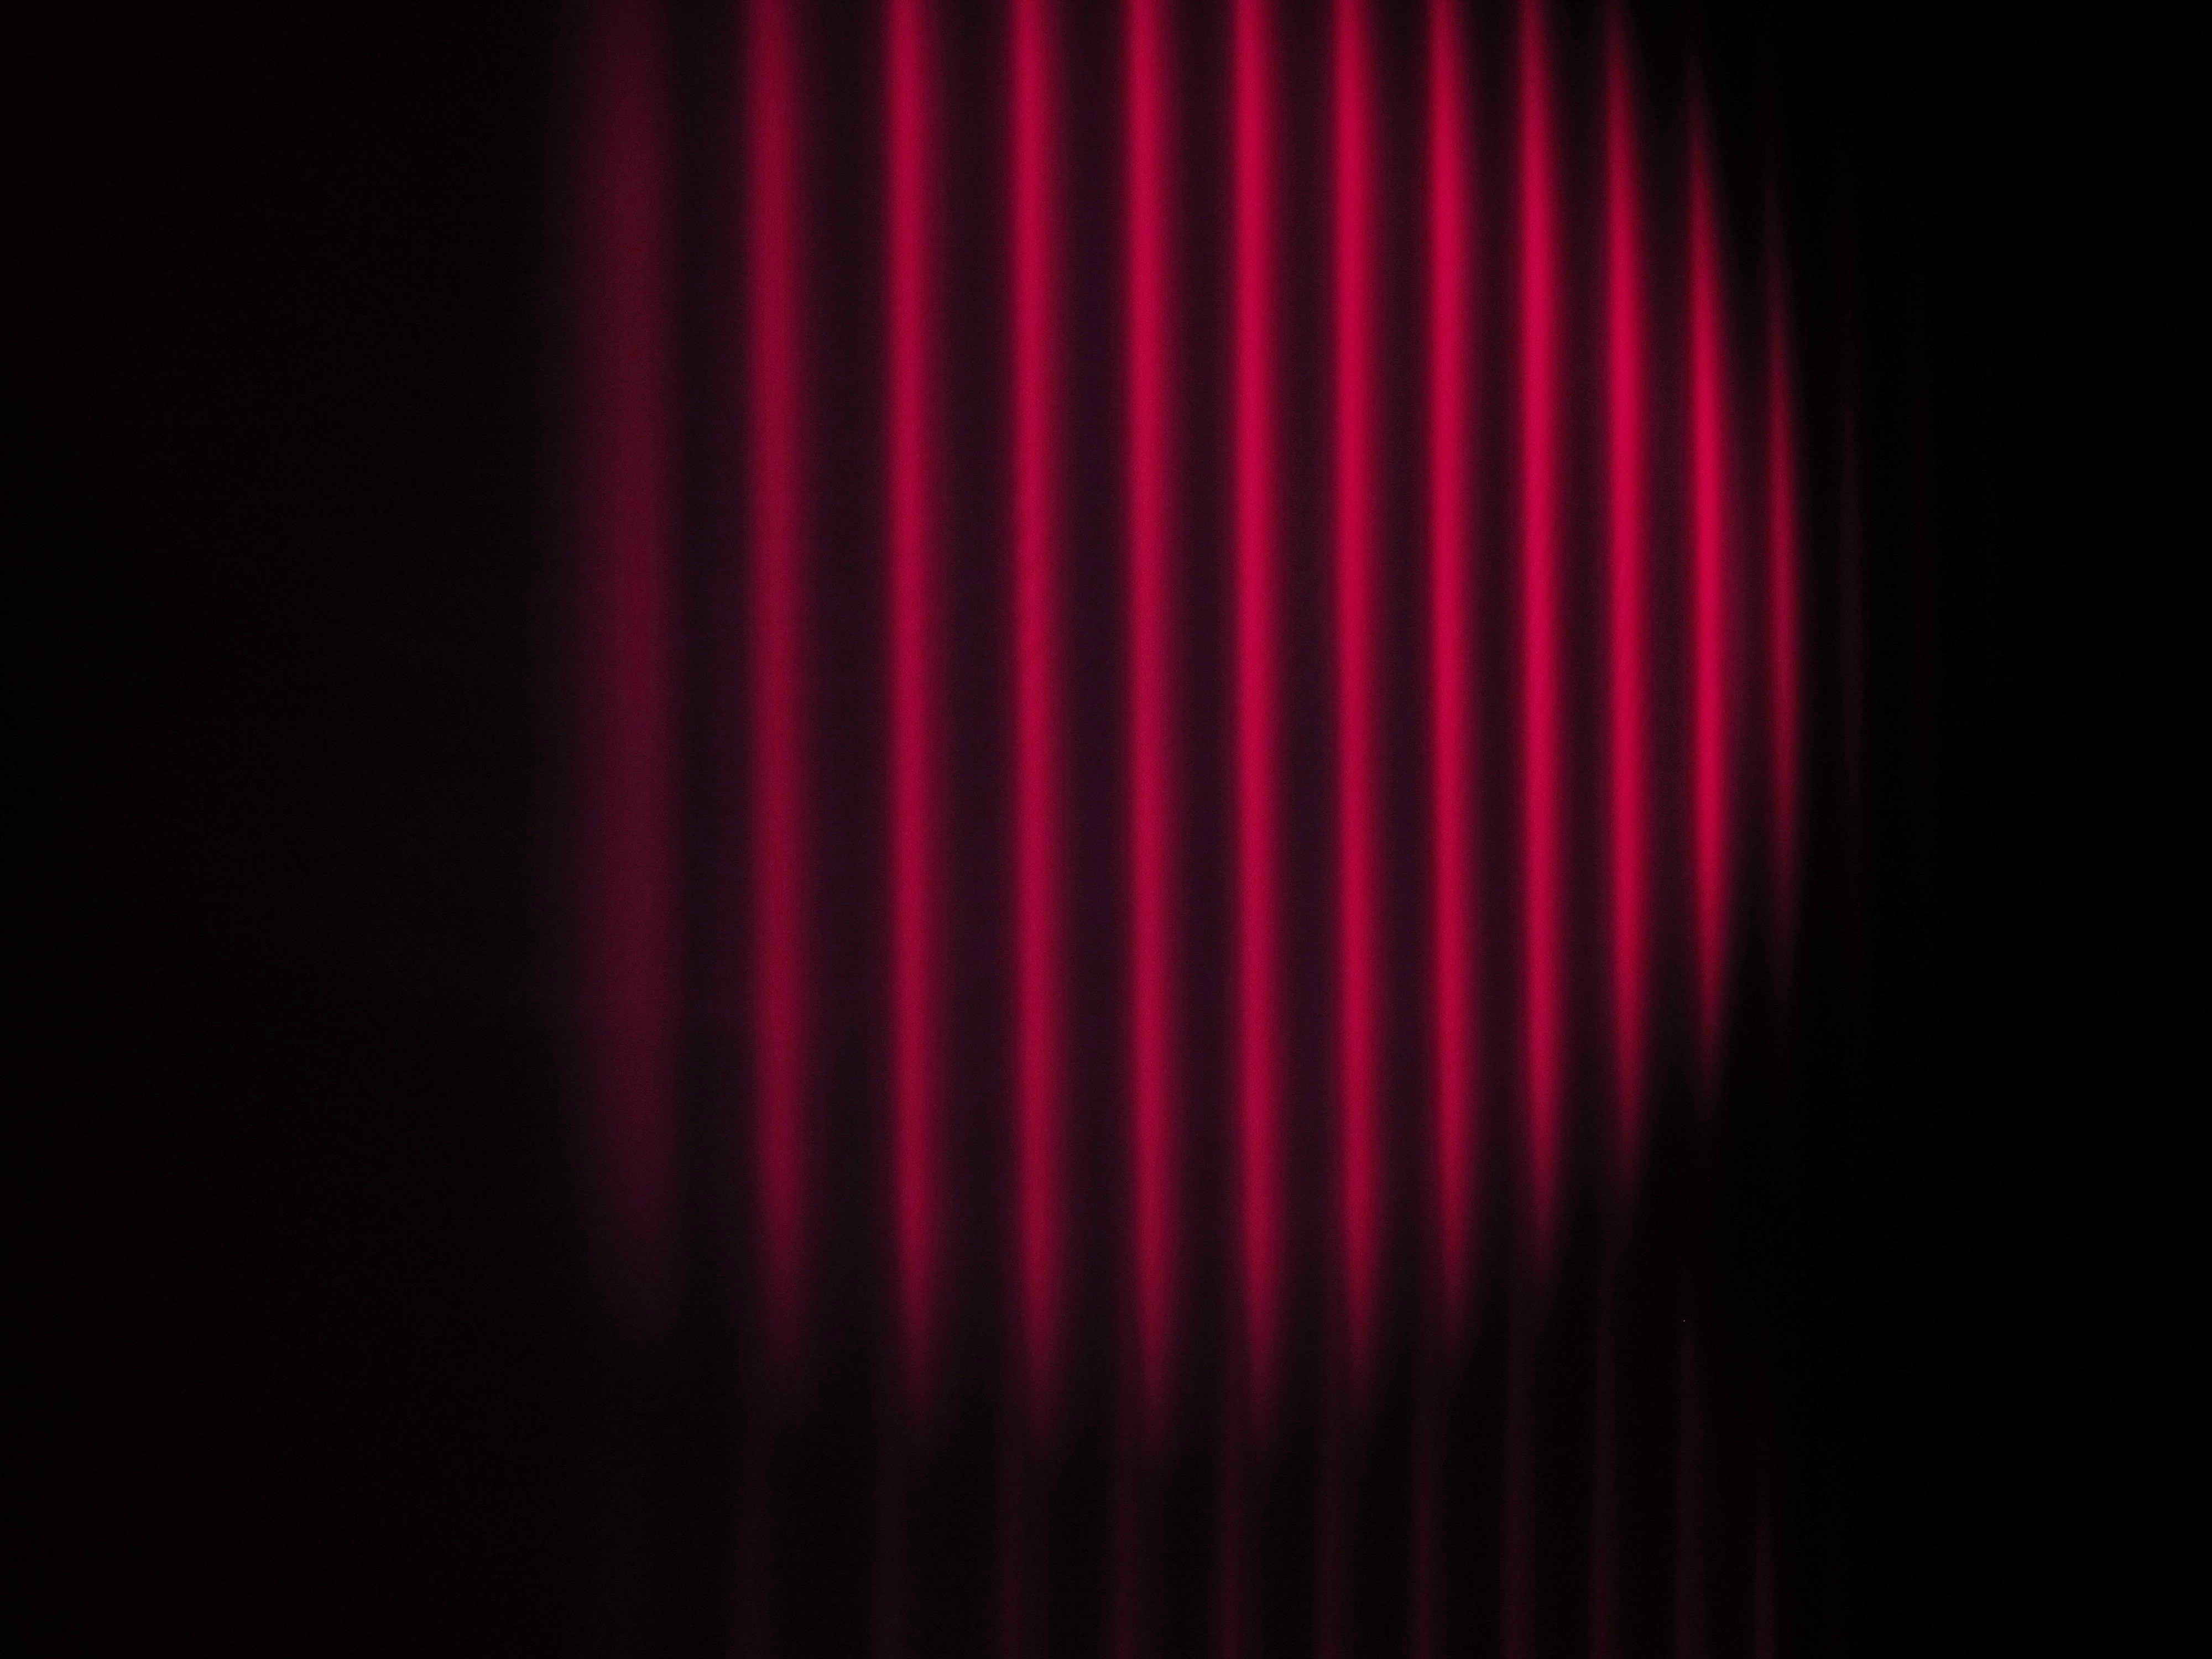
\includegraphics[width=0.95\textwidth]{data/temp/rot_mitB_90_aufgehellt.JPG}
  \caption{Interferenzbild der Lummer-Gehrcke Platte für die rote Spektrallinie mit angelegtem Magnetfeld für die $\pi$-Polarisation, zur besseren Abstandsmessung mit GIMP aufgehellt.}
  \label{fig:rotMitB90_aufgehellt}
\end{figure}



\begin{figure}[h!]
  \centering
  
\includegraphics[width=0.85\textwidth]{data/temp/blau_ohneB_0.JPG}
  \caption{Interferenzbild der Lummer-Gehrcke Platte für die blaue Spektrallinie ohne angelegtes Magnetfeld für die $\sigma$-Polarisation.}
  \label{fig:blauOhneB0}
\end{figure}
\begin{figure}[h!]
  \centering
  
\includegraphics[width=0.95\textwidth]{data/temp/blau_mitB_0.JPG}
  \caption{Interferenzbild der Lummer-Gehrcke Platte für die blaue Spektrallinie mit angelegtem Magnetfeld für die $\sigma$-Polarisation.}
  \label{fig:blauMitB0}
\end{figure}

\begin{figure}[h!]
  \centering
  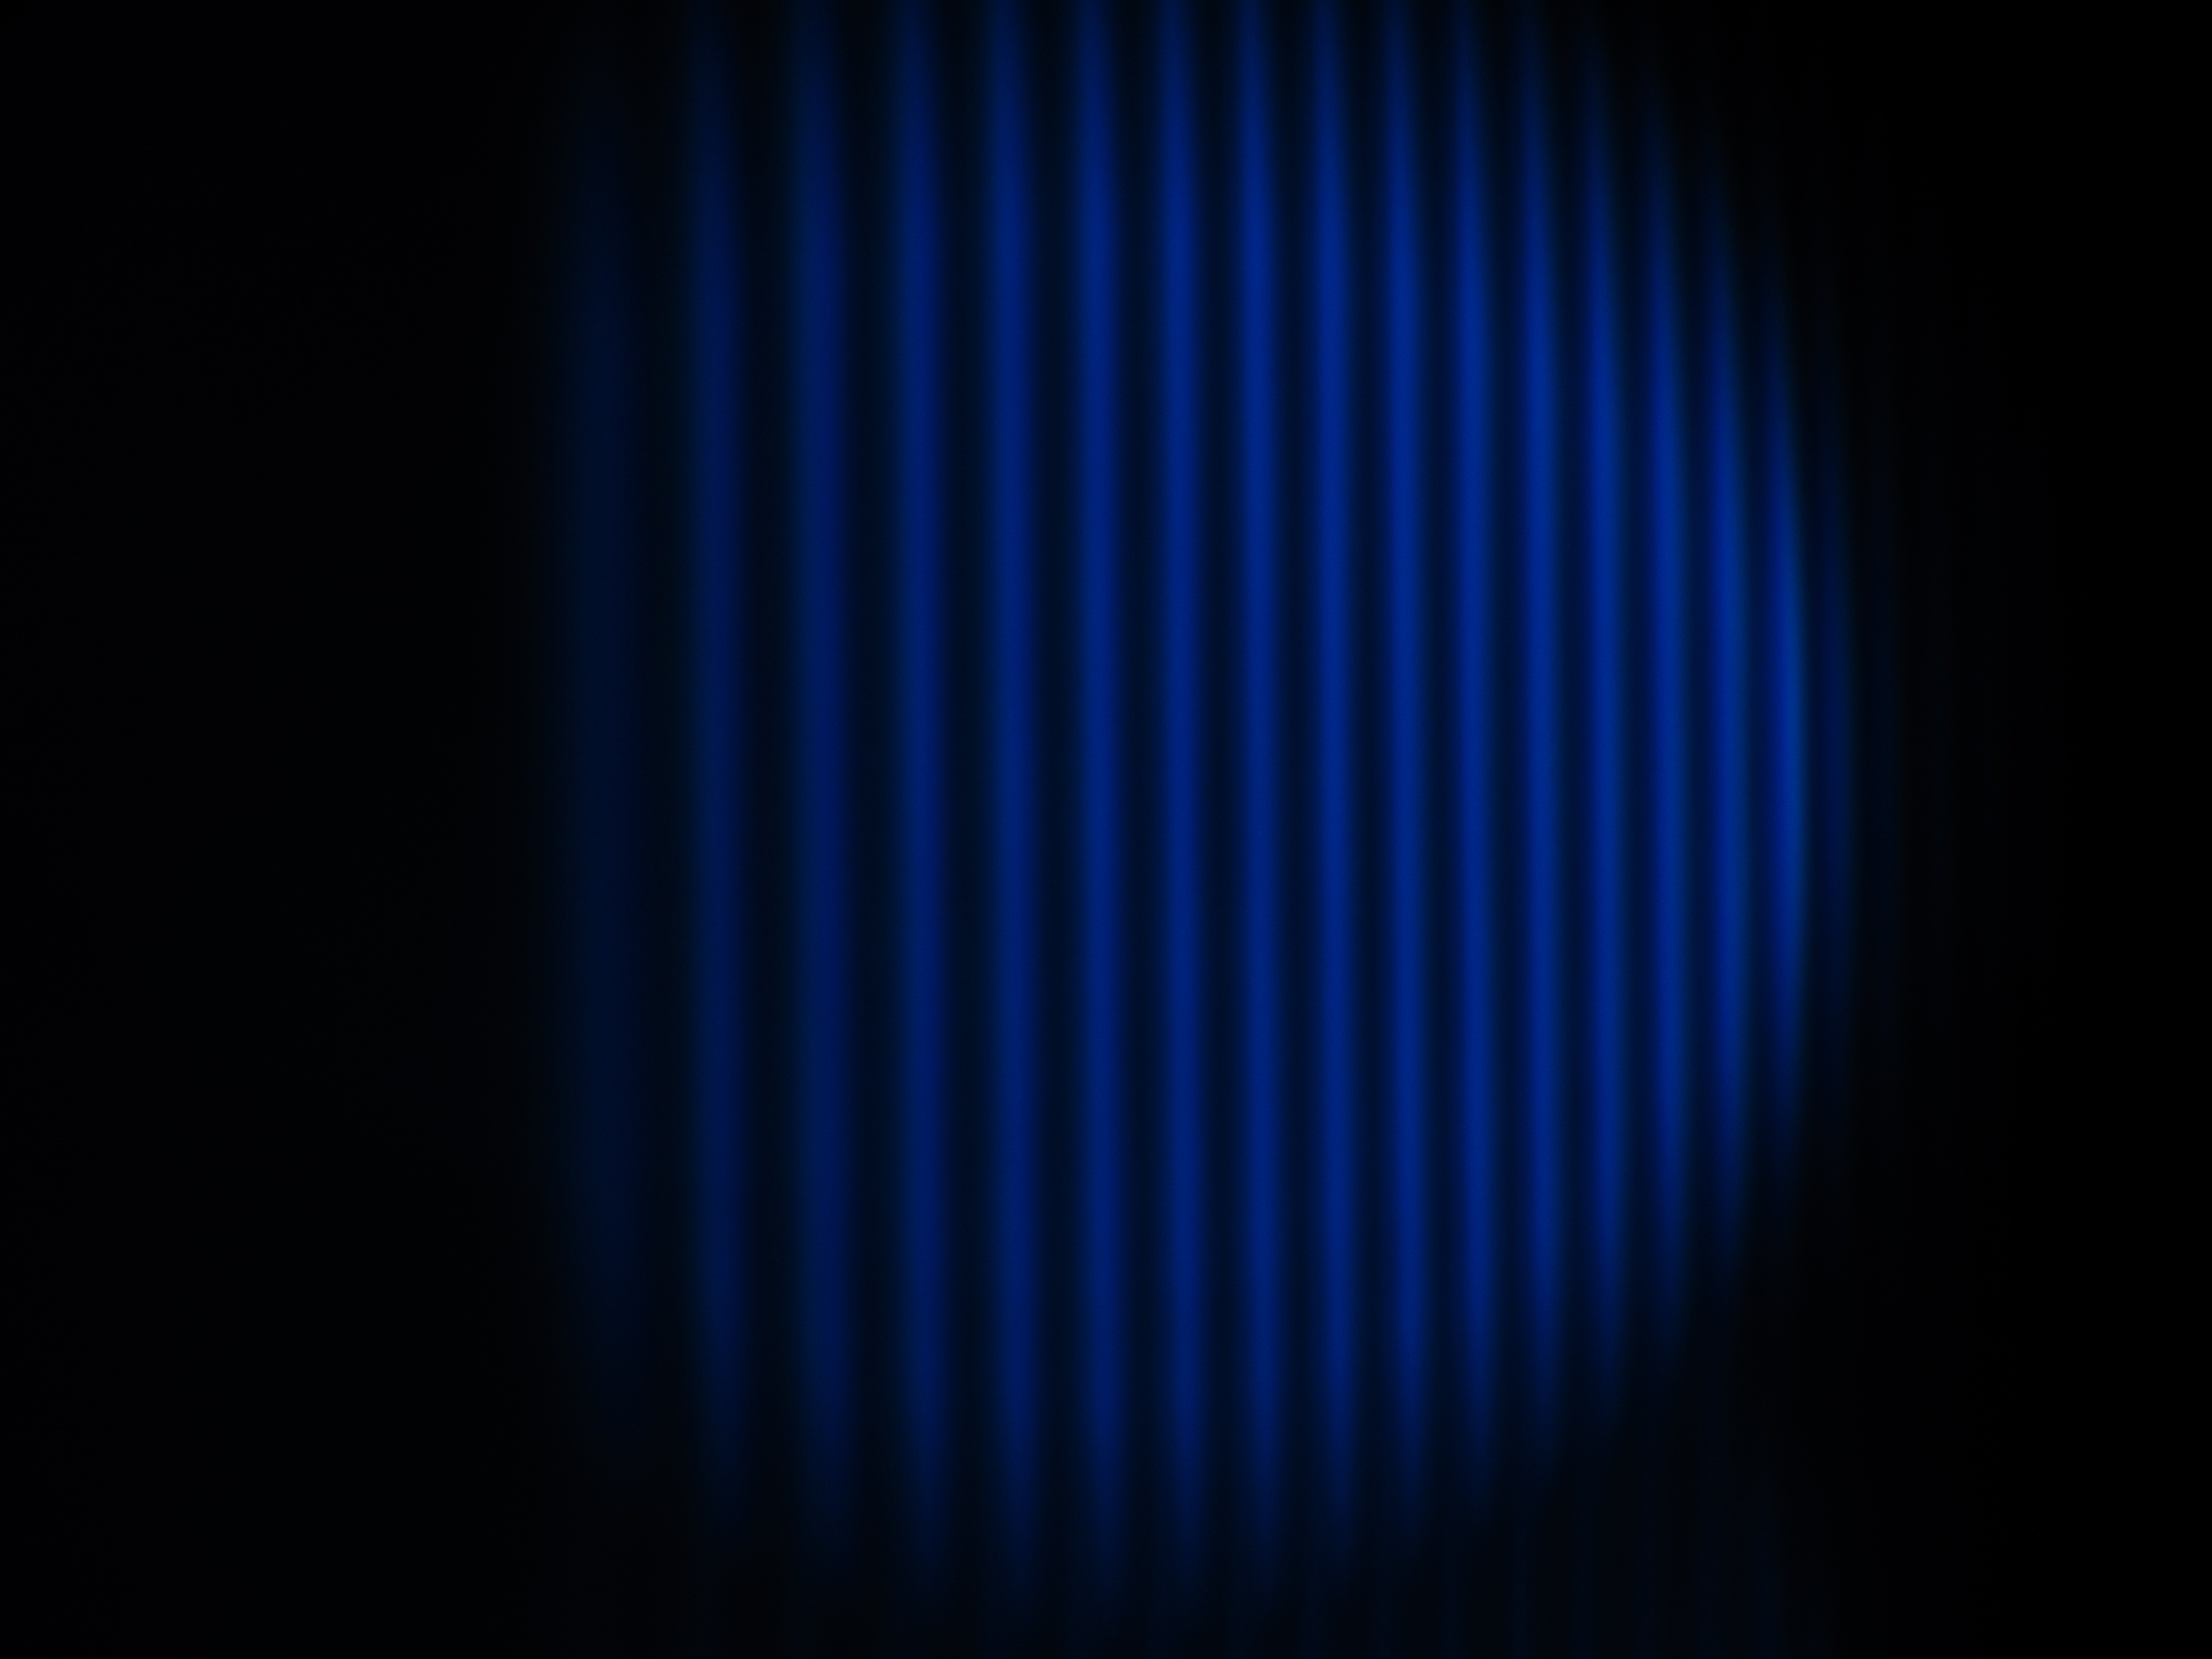
\includegraphics[width=0.85\textwidth]{data/temp/blau_ohneB_90.JPG}
  \caption{Interferenzbild der Lummer-Gehrcke Platte für die blaue Spektrallinie ohne angelegtes Magnetfeld für die $\pi$-Polarisation.}
  \label{fig:blauOhneB90}
\end{figure}
\begin{figure}[h!]
  \centering
  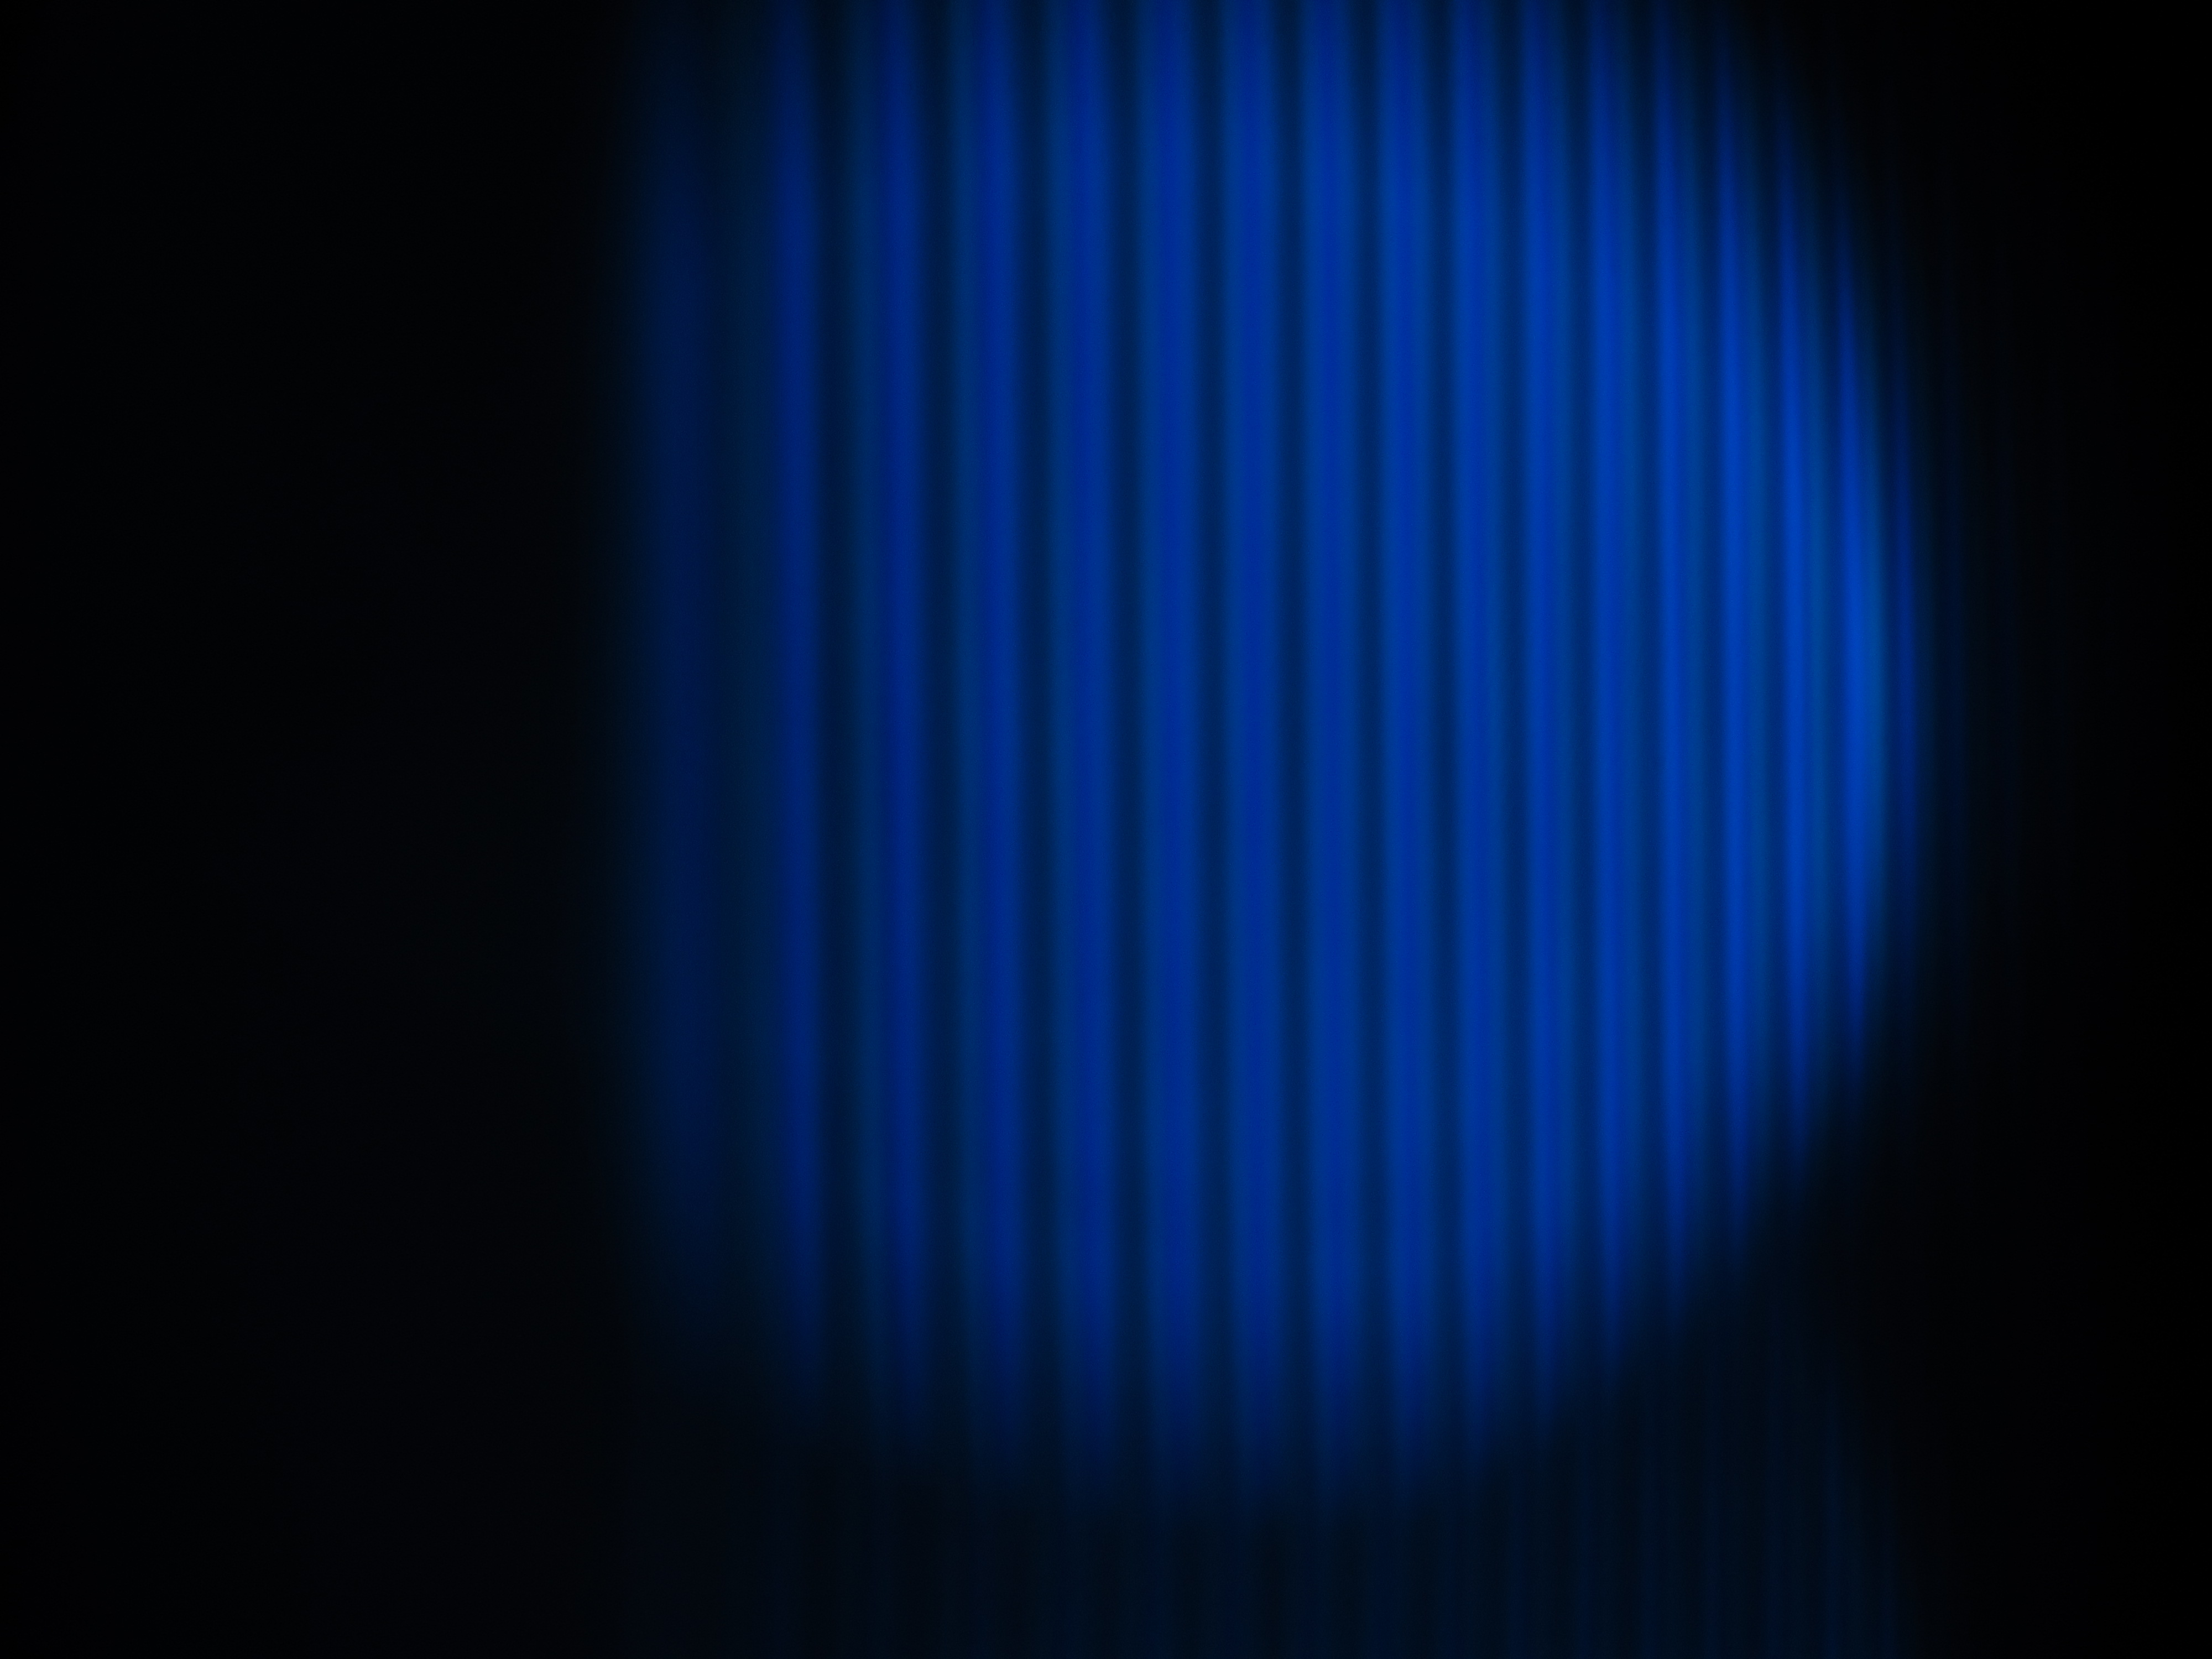
\includegraphics[width=0.95\textwidth]{data/temp/blau_mitB_90.JPG}
  \caption{Interferenzbild der Lummer-Gehrcke Platte für die rote Spektrallinie mit angelegtem Magnetfeld für die $\pi$-Polarisation.}
  \label{fig:blauMitB90}
\end{figure}
